% Stage report V: English edition. Build: pdflatex stage_report_5.tex (twice).
% Number provenance and independent verification: verified_numbers.json and README.md in this folder.
\documentclass[11pt,a4paper]{article}
\usepackage[margin=0.9in]{geometry}
\usepackage{amsmath,amssymb,booktabs,tabularx,array,graphicx,xcolor,float}
\usepackage[hidelinks]{hyperref}
\usepackage{enumitem}
\setlist{itemsep=3pt,topsep=5pt}
\renewcommand{\refname}{References}
\newcolumntype{Y}{>{\raggedright\arraybackslash}X}
\newcommand{\code}[1]{\nolinkurl{#1}}
\emergencystretch=3em
\linespread{1.15}
\setlength{\parindent}{0pt}
\setlength{\parskip}{5pt}
\title{\bfseries The typing gap, the candidates and the labels: ceiling diagnostics,\\consensus audits and a pre-registered utility-learning stop\\[7pt]
\large PanNuke nuclei instance segmentation: stage report V}
\author{Course project bdd26}
\date{October 13, 2026\\\small Experiments covered: October 9--12, 2026}
\begin{document}
\maketitle

\begin{abstract}
Stage report IV left two questions open: how much of the gap between official mPQ (0.4995) and class-agnostic bPQ (0.6653) is recoverable learning signal, and what the unmatched candidates added by the cross-scale arm actually are --- in particular, whether the labels themselves are trustworthy. This stage answers both with five experiments. A typing-oracle diagnostic shows that retyping every matched instance to its ground-truth class, with geometry untouched, would lift three-split mean mPQ to 0.6632, with about 70\% of the gain associated with Inflammatory/Connective ground truth. The pre-registered probe T0--T3 then tests whether simple read-outs can cash in any of that headroom: the best configuration gains $+0.0002$ (CI straddling zero) and the unweighted linear head loses $0.0053$ Dead PQ, tripping the guard-rail; post-hoc retyping of frozen features is closed as a line. The independent human audit became unavailable (no expert resources), so E1 was executed in its approved no-expert revision: a 13-seat cross-fold detector jury supports frozen candidates far above a synthetic null control ($\geq$3-seat support in 0.75\% of random blobs versus 66--73\% of zero-overlap candidates), and support is monotone in ground-truth match rate; two model pre-review passes disagree with each other (kappa $-0.09$ to $+0.35$) and are unusable. Building on this, the E1-T typing-consensus audit finds that on instances the base model mistyped, the 12-seat jury majority agrees with the \emph{base} class on 72.5\% [0.706, 0.742] of cases against 18.2\% for the ground-truth class (CI-separated), while the jury's intrinsic flip rate on correctly typed instances is 1.9\% --- the pre-registered key for Inflammatory/Connective label-boundary ambiguity is met, as detector-resonance evidence rather than a biological claim. Finally, E3 folds jury support into candidate-quality learning: utility itself is cheaply predictable (CV AUC 0.721/0.737), but under the frozen selection rule every learned row is rejected by the strict-Dead floor and the line closes by pre-registered stop rule. Four of the five experiments are CPU-only replays that never read a test fold; the oracle diagnostic is read-only audit access to already-evaluated test predictions. The suite passes 335 tests; final artifacts were regenerated bit-exact after independent review.
\end{abstract}
\noindent\textbf{Keywords:} nuclei instance segmentation; PanNuke; label noise; detector consensus; pre-registered gates; candidate filtering

\section{Background and questions for this stage}

Stage report IV settled the mechanism and the cost of the cross-scale candidate arm\cite{reports}: the HV area threshold explains only a small part of the $2\times$ Dead gain, the Dead-specialist branch closed under its gradient-conflict gate, and the two-model system costs about 6.1$\times$ single-model inference. EF-P2 remains mechanism evidence and a teacher candidate. After that, the research questions became more basic than ``one more detection improvement''.

\textbf{The typing gap.} The CellViT-UNI baseline scores 0.4995 official mPQ against 0.6653 bPQ. A substantial share of already-detected nuclei is mistyped. The earlier CONCH re-typing null\cite{structure} ruled out external vision--language features, but the model's own frozen features had never been probed for extractable typing signal.

\textbf{Candidates and labels.} Between 53 and 61\% of the candidates added by EF-P2 match no ground-truth instance (55.9\% on the validation fold; 57--61\% under the historical test-fold convention). Debris, contour disagreement and genuinely unlabelled nuclei all produce the same observable. The October 9 proposal\cite{next} therefore planned two parallel tracks: a fixed-geometry typing probe (T) and an independent candidate audit (E1).

The stage took one more turn than planned. After T failed its gate, E1 lost its human reviewers (resource unavailability confirmed on October 11), and the approved no-expert revision spawned two further pre-registered experiments\cite{specs}: the E1-T typing-consensus audit and the E3 candidate-quality dev round. The sections follow chronology: Section~\ref{sec:oracle} the ceiling diagnostic, Section~\ref{sec:t} the probe, Section~\ref{sec:e1} the packet and the no-expert revision (E1-C/E1-M), Section~\ref{sec:e1t} E1-T, Section~\ref{sec:e3} E3, and Section~\ref{sec:verify} the verification record.

Data boundaries follow the previous stage. T, E1-C, E1-M, E1-T and E3 use training and validation folds only and read no test fold; apart from two HoVer-Net validation-fold inferences added for the E1-C jury, there is no new GPU work and no training anywhere in this stage. The one exception is the ceiling diagnostic of Section~\ref{sec:oracle}, which reads frozen, already-evaluated three-split test predictions as audit-type access --- read-only, no tuning --- and is flagged as such.

\section{Typing-oracle ceiling}\label{sec:oracle}

The diagnostic answers a plain question: if every detected nucleus were given its correct class, where would the score sit? We read the frozen baseline test predictions (no TTA, last checkpoint), keep instance counts and contours exactly fixed, replace the class of every IoU$>$0.5 matched instance with its ground-truth class, and re-score mPQ with the canonical evaluator\cite{structure}. Such ground-truth-assisted interventions are oracles: they bound what perfect typing could add to the \emph{current} geometry, and are not achievable performance.

\begin{table}[H]
\centering\small
\caption{Typing-oracle interventions (three-split means; geometry fixed, only matched instances retyped). The third row retypes matched instances whose ground truth is Inflammatory or Connective, regardless of the predicted class.}
\label{tab:oracle}
\begin{tabular}{lrr}\toprule
Intervention & mean mPQ & vs.\ current\\\midrule
Current classes & 0.49951 & ---\\
All matched instances retyped to GT & 0.66322 & $+0.16371$\\
GT-Infl/Conn matched instances retyped to GT & 0.61412 & $+0.11461$\\
\bottomrule
\end{tabular}
\end{table}

Per-split gains are $+0.169/+0.167/+0.155$, all in the same direction. The split-1 per-class moves (current$\to$oracle) are Neoplastic $0.570\to0.666$, Inflammatory $0.440\to0.720$, Connective $0.418\to0.595$, Dead $0.142\to0.411$, Epithelial $0.575\to0.659$. Inflammatory and Connective move most; Dead has the largest absolute headroom but stays bounded by detection, since unmatched nuclei cannot be retyped.

The third row accounts for about 70\% of the second row's gain, and this share must be worded carefully: the script selects on \emph{ground-truth} class only, so it includes these two classes being confused with any other class, and each correction also removes false positives from the previously predicted class. mPQ is non-linear; 70\% is not an additive confusion decomposition\cite{structure}. Likewise the numerical proximity of oracle mPQ (0.6632) and bPQ (0.6653) is coincidence, not an identity --- the two metrics match and aggregate differently.

The diagnostic read historical test artifacts and was not pre-registered; it may propose hypotheses only. The hypothesis it proposes is direct: the typing gap is worth probing, with the Inflammatory/Connective boundary as the first suspect. The remaining sections test this line on validation data.

\section{T0--T3: the fixed-geometry typing probe}\label{sec:t}

\subsection{Design and gate}

The probe's hypothesis\cite{specs}: with nucleus count and contours untouched, instance-level features may still carry class information that the pixel majority vote does not use. Development is confined to split 1 --- fold 1 (63,218 GT instances) trains the read-out, fold 2 (59,593 predicted instances) validates, fold 3 is never read. Four configurations were frozen before any run: T0 majority vote (identity), T1 instance-mean class probability, T2 pooled frozen TP features with a linear head, T3 T2 plus a 24-px context ring at matched dimensionality.

\begin{table}[H]
\centering\small
\caption{T0--T3 validation-fold results (mPQ, difference vs.\ T0). Brackets are paired-image bootstrap 95\% intervals.}
\label{tab:t}
\begin{tabular}{llrr}\toprule
Config & Content & mPQ & $\Delta$ vs T0\\\midrule
T0 & pixel majority (current decode) & 0.483486 & ---\\
T1 & instance-mean probability & 0.483182 & $-0.0003$ [$-0.0010,+0.0003$]\\
T2 & pooled tp\_feat + linear head & 0.483707 & $+0.0002$ [$-0.0027,+0.0019$]\\
T3 & T2 + 24-px context ring & 0.481796 & $-0.0017$\\
\bottomrule
\end{tabular}
\end{table}

T0 reproduces the official fold-2 evaluation exactly. T2 reports the mean of two linear-head seeds (0.483606/0.483807), same direction. The gate required all six conditions simultaneously: $\Delta$mPQ $\geq+0.003$, interval lower bound above zero, strict mPQ not down, Dead PQ down by at most $0.002$, beating T1, and seed consistency.

\subsection{Verdict: gate failed}

Three of six conditions pass. The $+0.0002$ point estimate is far below the $0.003$ threshold and the interval lower bound is $-0.0027$; the decisive failure is the guard-rail --- the unweighted linear head loses $0.0053$ Dead PQ, beyond the $0.002$ allowance. A cheap read-out does not merely fail to help; it further starves the rarest class. The sklearn deterministic cross-check agrees in direction (0.4817, worse). Under the pre-registered rule no bigger classifier and no added configuration may rescue the result.

The failure position is visible in three accuracies. The linear head's diagnostic accuracy on \emph{ground-truth regions} is 85.3\%; its typing accuracy on \emph{matched predicted instances} is 85.8\%; the incumbent majority vote on the same population is about 85.7\%. The three coincide: the head extracts the same information the TP branch already uses. GT-feature export costs 790\,ms/image unoptimized, so there is no deployment case either. T1's $-0.0003$ shows the aggregation rule itself is saturated.

Combined with the CONCH null, two independent feature sources (an external pathology VLM; the model's internal frozen features) both fail post-hoc instance-level retyping. The bPQ--mPQ gap cannot be cashed in by changing the read-out. This leaves label ambiguity and joint training as the surviving explanations --- the first is tested by E1-T in Section~\ref{sec:e1t}; the second stays deferred.

\section{E1's turn: from human audit to detector consensus}\label{sec:e1}

\subsection{Packet and original protocol}

The pre-registered E1 packet\cite{specs} was built and frozen before anything else happened: 200 windows, 50 per source --- x1-detected objects (S1), EF-P2 accepted additions (S2), rejected candidates (S3) and random background (S4) --- stratified by tissue and border status with recorded inclusion probabilities; stage 1 shows image and cross-hair only, stage 2 reveals candidate and GT contours; the analysis script was committed before any reviewer answer existed. On October 11 the user confirmed that qualified human reviewers are unavailable for the foreseeable future. The human path is therefore \emph{not executed but not voided}: the packet is unchanged, the obligation is recorded, and the original protocol can run verbatim if reviewers ever materialise.

With user approval, E1 proceeded in its no-expert revision (spec~\S7): cross-detector consensus (E1-C) in place of biological judgement, and a non-expert model pre-review (E1-M) to test whether the cheap option is even usable. Both yield \emph{detector-level evidence only} and make no biological claims.

\subsection{E1-C: cross-detector consensus with a null control}

The jury has 13 seats: split-1/split-3 $\times$ three seeds $\times$ \{x1, x2\} of CellViT (11 seats) plus two HoVer-Net seats (split 1/split 3, fold-2 inference, validation-fold sanity mPQ 0.4509). No member ever trained on fold 2. Candidates are the frozen split1\_seed1 eligible pool of 4,084 (1,515 accepted, 2,569 rejected); support counts members overlapping a candidate at IoU$\geq0.3$.

Consensus needs a calibration point. The synthetic null control\cite{specs} places same-area discs at random positions outside an 8-px dilation of all GT instances (areas resampled from the zero-overlap candidate distribution; $n=2{,}000$): mean support 0.07, $\geq3$-seat rate 0.75\%, $\leq1$-seat rate 99.1\%. Random placement almost never manufactures agreement. This controls the random baseline only --- not detector-family-shared false-positive modes.

\begin{table}[H]
\centering\small
\caption{E1-C: ground-truth match rate (IoU$>$0.5) by binned jury support.}
\label{tab:e1c}
\begin{tabular}{lrrrr}\toprule
Group & n & mean support & match rate, support 0--2 & match rate, support $\geq$5\\\midrule
S2 (EF-P2 accepted) & 1,515 & 5.47 & 9.6\% & 55.3\%\\
S3 (EF-P2 rejected) & 2,569 & 5.04 & 8.5\% & 45.0\%\\
Synthetic null & 2,000 & 0.07 & \multicolumn{2}{c}{$\geq3$-seat rate 0.75\%}\\
\bottomrule
\end{tabular}
\end{table}

\begin{figure}[H]
\centering
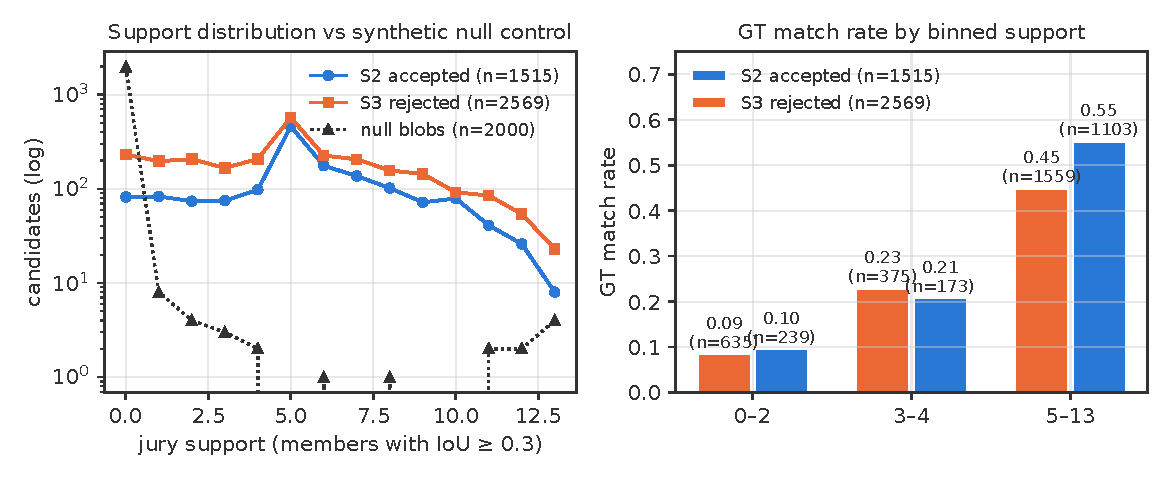
\includegraphics[width=\linewidth]{figs/e1c_support_en.pdf}
\caption{E1-C support distribution and GT match rate by binned support. Left: candidate support concentrates at 5--7 seats while the synthetic null stays at 0--1 (log axis). Right: GT match rate rises monotonically with support.}
\label{fig:e1c}
\end{figure}

Candidates cluster at 5--7 seats regardless of the EF verdict, two orders of magnitude above the null, and match rate is monotone in support. Stratifying by the GT relation sharpens the picture:

\begin{itemize}
\item \textbf{Zero overlap with GT} (S2 518, S3 1,146): mean support 4.8/4.4, and $\geq$3 seats with cross-fold \emph{and} cross-architecture support on 380 (73.4\%) and 751 (65.5\%) respectively. Detectors trained on disjoint folds from two architectures generalize only from labelled nuclei; consistent nucleus-shaped detections where the labels have nothing constitute \emph{detector-resonance evidence that the labels are suspect}. Candidate explanations --- annotation-unit differences, skipped degenerate/apoptotic objects, family-shared false-positive modes --- are not distinguished here.
\item \textbf{Overlap but below the match line} ($0<\text{IoU}\leq0.5$; S2 328, S3 582): support is similarly high, consistent with a contour/instance-unit disagreement subpopulation --- the object is seen, but bounded differently from the annotation.
\item \textbf{Debris-compatible} (support $\leq1$) unmatched candidates: 10.0\% of S2 and 15.5\% of S3. The EF area filter points the same way but separates this subgroup only weakly.
\end{itemize}

The engineering consequence was written down the same day: support is a strong, monotone, null-calibrated predictor of candidate quality, so candidate-quality learning with low-dimensional features plus jury support now has an evidence base --- which is exactly what E3 (Section~\ref{sec:e3}) tests. Limitations as recorded: a single candidate pool (split1\_seed1); CellViT holds 11 of 13 seats, so cross-architecture evidence rests on two HoVer-Net seats; the null control uses synthetic discs, not nucleus-shaped probes.

\subsection{E1-M: model pre-review is unusable}

The packet's 200 windows also tested whether vision models can serve as reviewers. Two independent blind passes (an image-analysis channel, passA, and another model's native vision, passB) were both labelled by non-expert models. PassA judges only 40.9\% of S1 --- x1-detected objects, almost all genuine nuclei --- as real, a systematic non-nucleus bias with templated rationales. PassB ranks sensibly (S1 91.5\% $>$ S2 50.6\%/S3 57.3\% $>$ S4 40.8\%) but returns uncertain on 34--70\%. Between the two passes, raw agreement is 0.18--0.38 and kappa is $-0.09$ to $+0.35$: \emph{the model reviewers cannot even agree with each other}. E1-M fulfils its process-validation purpose only, and retroactively supports the spec's decision to exclude model review from formal conclusions.

\section{E1-T: typing consensus and the label boundary}\label{sec:e1t}

\subsection{Design and pre-registered key}

The first surviving explanation from T's failure was Inflammatory/Connective label ambiguity. E1-T\cite{specs} tests it with E1-C's epistemics: on instances the base model (split1\_seed1, x1, identity decode) \emph{mistyped}, do detectors that never saw this prediction systematically side with the base class over the ground-truth class?

The jury is E1-C's 13 seats minus the base run itself: 12 seats (CellViT 10 + HoVer-Net 2, training folds \{1, 3\}). Everything is a CPU replay of cached predictions, reading fold 2 only. Instance pairing follows the official evaluator (greedy IoU$\geq0.5$); a member's type vote for a GT instance is the pixel-majority class of its maximum-IoU instance when that IoU is $\geq0.3$. The majority class is defined with no reference to base or GT: at least 3 total votes, a strict plurality, and top-class votes from both training folds; otherwise ``no majority''. Groups: G1 = base mistyped (6,858), G0 = base correct (40,558); unmatched GT 12,456 and zero ambiguous complete the 59,872 GT instances of fold 2, verified against the fold total.

The pre-registered interpretation key: if, on G1's Infl/Conn cells, P(majority $=$ base) exceeds P(majority $=$ GT) with cluster-bootstrap separation and exceeds the G0 intrinsic flip rate, then ``Inflammatory/Connective label-boundary ambiguity (detector-resonance evidence)'' holds and the typing gap contains a component not removable under the current labels; otherwise the gap is recorded as model limitation and joint training stays deferred. Dead cells are reported separately whatever their direction.

\subsection{Result: the jury sides with the base model}

\begin{table}[H]
\centering\small
\caption{E1-T headline results. Brackets are image-cluster bootstrap 95\% intervals (2,000 draws, seed 20261011).}
\label{tab:e1t}
\begin{tabular}{lrr}\toprule
Statistic & Rate & 95\% CI\\\midrule
G1: majority $=$ base class & \textbf{72.5\%} (4,970/6,858) & [0.706, 0.742]\\
G1: majority $=$ GT class & 18.2\% (1,246/6,858) & [0.167, 0.197]\\
G1: majority $=$ other class & 3.6\% (247) & ---\\
G1: no majority & 5.8\% (395) & [0.052, 0.064]\\
G0: majority $\neq$ GT (intrinsic flip rate) & \textbf{1.9\%} (767/40,558) & [0.017, 0.021]\\
\bottomrule
\end{tabular}
\end{table}

\begin{figure}[H]
\centering
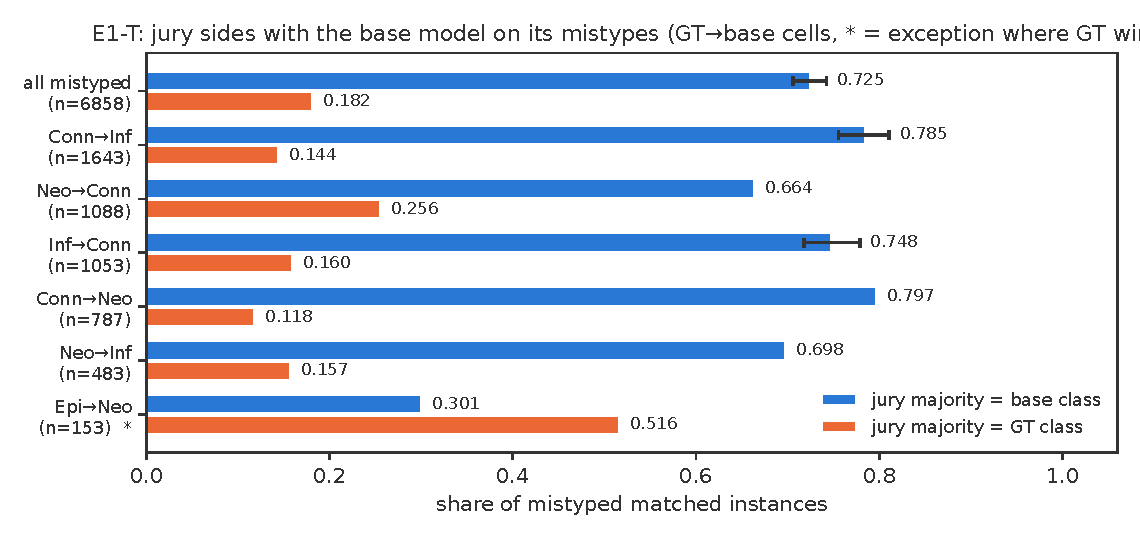
\includegraphics[width=\linewidth]{figs/e1t_pairs_en.pdf}
\caption{E1-T jury-majority allegiance on the largest (GT$\to$base) cells. The first three rows carry bootstrap intervals (whiskers). Epi$\to$Neo (starred) is the only large cell where GT wins.}
\label{fig:e1t}
\end{figure}

On G1 the jury majority equals the base class on 72.5\% of instances against 18.2\% for the GT class, CI-separated, while on G0 --- where base and GT already agree --- the jury flips only 1.9\%. G0 constrains the pure-echo explanation: an oracle-copying jury would show $\approx$0\% flips on G0 and $\approx$100\% base agreement on G1; neither holds.

The (GT$\to$base) decomposition puts the Inflammatory/Connective pair on top: GT-Inf/base-Conn, 74.8\% [0.718, 0.779] for the base class over 1,053 instances; GT-Conn/base-Inf, 78.5\% [0.756, 0.811] over 1,643. The two large Neoplastic$\to$\{Inf, Conn\} cells point the same way (69.8\%/66.4\%). The single large exception is GT-Epi/base-Neo (153 instances), where GT wins (51.6\% vs.\ 30.1\%) and which is reported separately. Dead-related cells total 404 instances; majority $=$ base sits in [0.573, 0.703] against [0.173, 0.282] for GT --- same direction, lower amplitude, heterogeneous within cells, and per the spec descriptive only.

Three sensitivity variants agree in direction: pairing threshold IoU 0.5 gives 72.0\%; minimum votes 5 gives 72.3\%; the HoVer-Net-only two-seat sub-jury gives base 36.0\% vs.\ GT 20.2\% (no-majority 36.2\%, G0 flip 6.7\%) --- weaker, not reversed, on the only cross-architecture subset.

\subsection{Conclusion and boundary}

Under the pre-registered key, \emph{Inflammatory/Connective label-boundary ambiguity is supported as detector-resonance evidence}. The result interlocks with T0--T3 and the CONCH null: post-hoc read-outs extract no increment not because the features are empty but because their ceiling is bounded by label noise --- where the jury consistently endorses the base class, supervision teaches the base answer as correct. The bPQ--mPQ typing gap therefore contains a component not removable under the current label supervision; the joint-training hypothesis stays deferred and is not activated by this result.

The boundaries are material. This is detector resonance, not biology: 10 of 12 jury seats share the CellViT recipe with the base model (the two HoVer-Net seats are the only cross-architecture control, and the signal weakens but holds there); one split, one base run; ``ambiguity'' is an interpretation of a statistical pattern, not an indictment of PanNuke's annotation process. Together with E1-C's existence-axis resonance this closes a two-axis label-quality evidence chain, but both axes stop at ``labels are suspect'' and do not quantify a noise rate.

\section{E3: candidate-quality learning, dev round}\label{sec:e3}

\subsection{Design and five-arm replay}

E1-C showed support to be monotone in candidate utility. E3\cite{specs} tests the stronger proposition: can a learned quality score replace the hand-written EF rule? Training data are 13,332 out-of-fold fold-1 candidates (generated by split-2 models across three seeds; fold 1 is their validation fold, so the candidates are out-of-fold) labelled by the frozen \code{matched} column. Application is the frozen split1\_seed1 pool of 4,084 candidates replayed on fold 2 in five arms: A0 identity; A1 frozen EF-P2 (incumbent, a30d); A2 pure area bands; A3 learned quality from 12 low-dimensional features (area, extent, circularity, distance, confidence, margin, border flag, class one-hot); A4 adding jury support. The model is logistic regression with hyperparameters chosen by grouped CV inside fold 1. Fold 3 is never read; fold-2 match labels appear in endpoints only.

Per-arm selection reuses the EF-round rule verbatim: among rows with mPQ and bPQ $\geq$ identity$-0.002$, strict Dead $\geq$ identity and interior-Dead matched above identity, take the highest validation mPQ. The A1 replay asserts against the frozen EF-P2 selection to $10^{-12}$; its a30 variant once reproduced the EF-round mPQ (0.48346) bit-exact, anchoring pipeline correctness.

The primary gate demands vs.\ A1: $\Delta$Dead $\geq+0.002$ with $\Delta$bPQ $\geq-0.0005$ and $\Delta$strict-Dead $\geq-0.002$; the secondary gate demands comparable Dead at $\geq$25\% fewer unmatched additions. Either gate passing opens a confirmation round; both failing closes the line with no menu extension and no model swap.

\subsection{Verdict: all three gates fail}

\begin{table}[H]
\centering\small
\caption{E3 key rows on fold 2. ``Best learned strict'' is the highest strict Dead among all A2--A4 rows; the descriptive row is the official-metric optimum.}
\label{tab:e3}
\begin{tabular}{lrrrrrr}\toprule
Row & mPQ & bPQ & Dead PQ & strict Dead & added & unmatched\\\midrule
A0 identity & 0.48221 & 0.65093 & 0.16104 & 0.12957 & 0 & ---\\
A1 frozen EF-P2 & 0.48346 & 0.65218 & 0.16714 & 0.13448 & 1,374 & 53.3\%\\
a4\_p0.7 (best learned strict) & 0.48395 & 0.65288 & 0.16547 & 0.12454 & 1,041 & 42.8\%\\
a4\_p0.5 (descriptive optimum) & 0.48487 & 0.65384 & 0.17011 & 0.12151 & 2,134 & 46.8\%\\
\bottomrule
\end{tabular}
\end{table}

\begin{figure}[H]
\centering
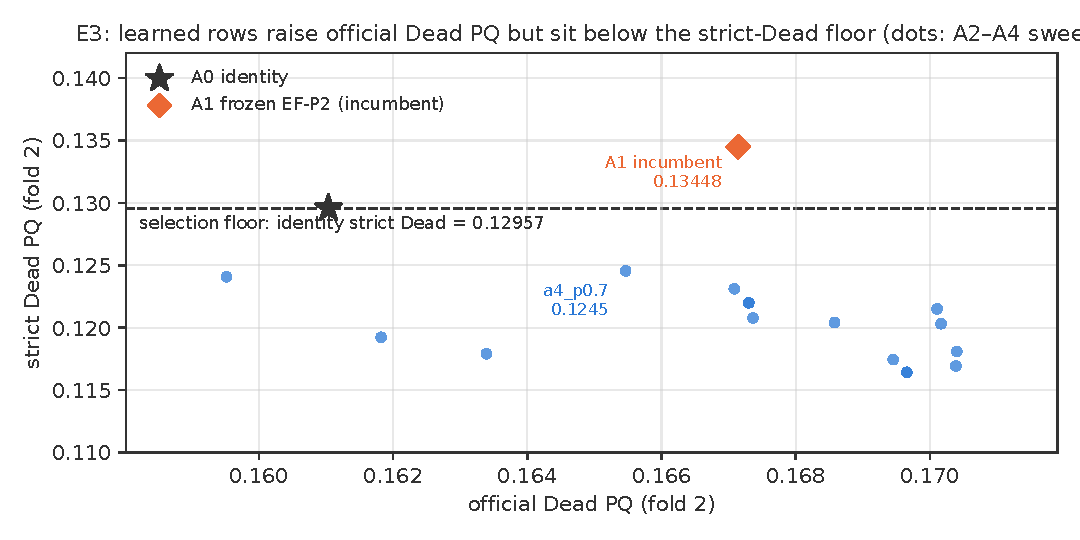
\includegraphics[width=\linewidth]{figs/e3_strict_en.pdf}
\caption{E3: official versus strict Dead PQ for all learned rows (A2--A4 menus). Learned rows do raise official Dead PQ, but every one sits below the identity strict-Dead floor; only the incumbent A1 clears it.}
\label{fig:e3}
\end{figure}

The selection rule rejected the learned rows in all 16 non-identity rows across A2--A4 --- not on official endpoints but on the strict-Dead floor: the best learned strict Dead is 0.12454 against identity's 0.12957, while A1 itself (0.13448) is one of the few rows that clear the bar. All three arms therefore fall back to identity, and the gate values are identity minus A1: $\Delta$Dead $-0.0061$, $\Delta$bPQ $-0.0012$, $\Delta$mPQ $-0.0012$ (bootstrap intervals at or below zero; mPQ $[-0.00242,-0.00014]$). Primary and secondary gates are false on every arm; the line closes under the pre-registered stop rule.

Where did it fail? Layer by layer:

\begin{enumerate}
\item \textbf{Utility is cheaply predictable.} Fold-1 grouped-CV AUC is 0.721 (12 features) and 0.737 (with support); the low-dimensional arm calibrates well on fold 2 (mean 0.45 $\to$ rate 0.49; 0.65 $\to$ 0.62). E1-C's monotonicity carries over to the learned model. This layer did not fail.
\item \textbf{The selection rule conflicts with the endpoint.} The frozen rule is intrinsically biased towards adding few candidates on the strict axis; score-ordered rows never clear the bar. The failure is not ``utility is unlearnable'' but ``candidate-level utility is not image-level strict risk''.
\item \textbf{The descriptive control locates the blind spot.} a4\_p0.5 beats A1 on every official metric ($\Delta$mPQ $+0.0014$, $\Delta$bPQ $+0.0017$, $\Delta$Dead $+0.0030$; 2,134 additions vs.\ 1,374 at a lower unmatched fraction, 46.8\% vs.\ 53.3\%) --- at strict Dead $-0.0130$. Cheap official-metric wins exist, and they are all paid for in Dead false positives on Dead-free images, which candidate-level features (area, shape, confidence, support) cannot see.
\item \textbf{The support arm's shift was measured.} Adding support lifts CV AUC by $+0.016$, but the fold-1 jury (6 CellViT seats; the HoVer-Net split-2 checkpoint was lost to disk cleanup, so the spec's seventh seat is absent --- a disclosed deviation) differs in composition from fold 2's 13-seat cross-fold/cross-architecture jury: on fold 2 the 0.84 confidence bin realises a 0.58 match rate. Calibration degrades and the AUC gain never reaches the endpoints.
\end{enumerate}

Mapped onto the October 9 proposal: the E1-supported candidate-quality-learning branch closes. A simple quality model, jury support included, cannot replace the EF rule on the joint official-plus-strict criterion. If the line ever reopens, what is missing is \emph{image-level class-absence risk features} (a per-image Dead prior, tissue conditioning) rather than a fancier candidate-level head --- a new testable explanation, not an automatic new project. EF-P2's positioning as mechanism evidence and teacher candidate is unchanged.

\section{Process record, verification and tests}\label{sec:verify}

Implementation followed test-first discipline; several real defects were caught by guards and assertions mid-run and fixed with regression tests before reruns. The consequential ones: a $\pm1$ class-index shift in the typing probe (cached label rows repaired deterministically, features byte-identical); a global instance-id LUT that cross-wired images in the retyped map (rebuilt per image); E1-T's majority semantics moved from unique-value to pixel majority (real data carries 164 untyped instances); two conditional-bootstrap defects in E1-T (out-of-group rows counted as 0 instead of NaN; group membership tested after the event) exposed by a miniature fixture; and E3's incumbent binding initially used the a30 row --- the bit-exact a30 replay revealed the incumbent is a30d, after which the floor was derived from the frozen selection file with an assertion.

After a whole-branch independent review, the final E1-T and E3 artifacts were regenerated: bit-identical to the first version (all of E1-T; all of E3 except the bootstrap mPQ column, whose convention was corrected to the official NaN exclusion, moving the identity$-$A1 $\Delta$mPQ interval from $[-0.00232,-0.00002]$ to $[-0.00242,-0.00014]$ without changing the conclusion). Provenance was completed (EF selection row, module fingerprints, fold-2 GT hash). The document-versus-artifact audit passed all 56 checks, with two descriptive numbers corrected against artifacts (the support-arm 0.84-bin realised rate is 0.58, not 0.55; the support AUC gain is $+0.016$, not $+0.017$). The full suite passes \textbf{335 tests} (a net gain of 58 this stage) on the unchanged pinned environment.

\section{Limitations and next steps}

\subsection{Limitations}

\begin{enumerate}
\item \textbf{Everything sits in one development environment.} T, E1-C, E1-M, E1-T and E3 all run on split 1's validation fold with a single base run (split1\_seed1); E3's training side covers three split-2 seeds but its application side is one candidate pool. All confidence intervals reflect image-sampling uncertainty only.
\item \textbf{Resonance is not biology.} The jury shares recipe and architecture family with the base model; the null control uses synthetic discs; both label-evidence axes establish ``suspect'', not a quantified noise rate, and cannot separate missed labels, unit disagreement and shared false-positive modes.
\item \textbf{E3 is a dev-round verdict.} ``All gates fail'' applies to the frozen menu and rule; it refutes ``cheap candidate-level features can replace EF'', not quality learning in general.
\item \textbf{The ceiling diagnostic read test artifacts.} Section~\ref{sec:oracle} accessed historical test predictions (read-only, untuned, no new inference); the other four experiments read no test fold. There are no new three-split test scores, and the historical caveat about test-fold reuse stands.
\item \textbf{HoVer-Net seats are incomplete.} The lost split-2 checkpoint left E3's fold-1 jury without a cross-architecture seat; E1-C/E1-T cross-architecture evidence rests on two seats.
\end{enumerate}

\subsection{Next steps}

With both learning lines closed as nulls and both label-evidence chains closed as positives, the candidates ordered by evidence strength:

\begin{enumerate}
\item \textbf{Write label ambiguity into the final report's analysis frame.} The Infl/Conn finding changes the default reading of the typing gap; the tissue$\times$class error decomposition should be presented against the resonance evidence rather than booked entirely as model loss.
\item \textbf{Image-level class-absence risk features.} E3's surviving explanation: predicting ``does this image contain this class'' may be closer to the strict-axis pain than predicting ``is this candidate a nucleus''. If pursued, a spec first (entry conditions, controls, stop rule), under this stage's pre-registration discipline.
\item \textbf{Joint training stays deferred.} It changes capacity, features and schedule at once; the label and feature explanations must both be excluded first, and the current evidence does not support starting.
\item \textbf{The human-review obligation stands.} The E1 packet is unchanged; two qualified reviewers could execute the original protocol verbatim, at which point resonance evidence and biological judgement can be compared directly.
\end{enumerate}

Until one of these is approved, no new training starts, and no selection rule is widened on the already-much-observed test images.

\section{Conclusion}

This stage moved both questions left by stage report IV to evidence-based answers.

First, \emph{the typing gap cannot be cashed in by post-hoc read-outs}. Ground-truth-assisted retyping would lift mPQ from 0.4995 to 0.6632, about 70\% of it associated with Inflammatory/Connective ground truth; yet fixed-geometry read-outs (aggregation, linear head, context ring) extract no increment and hurt Dead. E1-T then supplies the mechanism-level explanation: on the base model's mistypes the cross-fold, cross-architecture jury endorses the base class on 72.5\% [0.706, 0.742] against 18.2\% for GT, with a 1.9\% intrinsic flip rate on correct instances --- the pre-registered Inflammatory/Connective label-boundary-ambiguity key is met. The read-out ceiling is bounded by label noise; that component of the gap is not removable under current supervision.

Second, \emph{unmatched candidates are not noise, and utility --- though learnable --- cannot replace the rule}. Zero-overlap candidates carry $\geq$3-seat cross-fold/cross-architecture support at 66--73\% rates (null: 0.75\%), establishing resonance evidence on the existence axis as well; support is monotone in match rate, and the learned quality model reaches CV AUC 0.721/0.737. But under the frozen selection rule every learned row fails the strict-Dead floor, and official-metric gains are uniformly paid for in class-absence false positives; E3 closes by stop rule.

Process-wise: four of five experiments were CPU-only replays, the fifth added two validation-fold inferences; no test fold was read, nothing was trained; the suite passes 335 tests, final artifacts replay bit-exact after review, and the document-versus-artifact audit passes 56 checks. The paired nulls (read-out, utility) and positives (label evidence) point the project towards label-aware analysis framing and image-level risk features --- not more read-out heads or wider filtering menus.

\appendix
\section{Files, numbers and reproduction}

\subsection{Number verification}

All table numbers were exported from the five frozen artifacts by \code{scripts/report5\_numbers.py} (snapshot: \code{runs/analysis/report5\_numbers.txt}). \code{scripts/verify\_report5.py} independently recomputes and checks them from the rawest available artifacts --- including: oracle current values bit-identical to the official baseline evaluations; the T gate booleans re-derived from stored values; E1-C support histograms and match rates recomputed from \code{per\_candidate.npz} joined with the frozen candidate records; E1-M agreement and kappa recomputed from the two CSV passes; E1-T group counts summing to the fold-2 GT total with intervals bracketing point estimates; and the E3 selection rule replayed over all rows, matching the frozen selections --- and writes \code{verified\_numbers.json} in this folder. Bootstrap intervals are the frozen results and are not redrawn. The zero-overlap stratification in Section~\ref{sec:e1} is re-derived from \code{per\_candidate.npz} and the candidate records because \code{consensus.json} stores aggregates only.

Figures come from \code{scripts/make\_report\_figures5.py} on the same artifacts; their values match the frozen CSVs in \code{figs/}.

\subsection{Artifacts and commands}

\begin{table}[H]
\centering\footnotesize
\caption{Main artifacts, relative to the repository root; \code{runs/} is local and not distributed via Git.}
\begin{tabularx}{\linewidth}{lY}\toprule
Path & Role in this report\\\midrule
\code{runs/analysis/typing\_oracle\_20261009/} & ceiling-diagnostic table and per-class results.\\
\code{runs/analysis/typing\_probe\_20261010/} & T0--T3 endpoints, gate values, diagnostics.\\
\code{runs/analysis/e1\_packet\_20261010/} & blinded audit packet (200 windows, two-stage protocol, awaiting reviewers).\\
\code{runs/analysis/e1\_consensus\_20261010/} & E1-C consensus, null control, E1-M two-pass review.\\
\code{runs/analysis/e1t\_typing\_20261011/} & E1-T groups, per-pair tables, bootstrap, sensitivity.\\
\code{runs/analysis/e3\_quality\_20261011/} & E3 five-arm endpoints, selection replay, model diagnostics.\\
\code{runs/analysis/report5\_numbers.txt} & per-table number snapshot for this report.\\\bottomrule
\end{tabularx}
\end{table}

From the repository root with the pinned environment:
\begin{quote}\small
\texttt{python scripts/report5\_numbers.py}\\
\texttt{python scripts/verify\_report5.py}\\
\texttt{python scripts/make\_report\_figures5.py}\\
\texttt{python -m pytest -q}
\end{quote}
The verification scripts exit with an error status on missing artifacts or numeric mismatch and never modify experiment artifacts.

\begin{thebibliography}{9}
\raggedright
\bibitem{reports} Project bdd26. Stage reports III--IV: cross-scale candidate filtering and mechanism controls[R]. 2026-10-06/08. \code{docs/report/stage\_report\_3/}; \code{docs/report/stage\_report\_4/}.
\bibitem{next} Project bdd26. Next-step research plan: verify learnability before scaling (2026-10-09)[R]. \code{docs/RESEARCH\_NEXT\_2026-10-09.md}.
\bibitem{structure} Project bdd26. Model structure, experiment review and strategy (2026-10-09 revision)[R]. \code{docs/STRUCTURE\_AND\_STRATEGY\_2026-10-09.md}.
\bibitem{specs} Project bdd26. Pre-registered specs: typing probe T, blind audit E1 with no-expert revision, typing consensus E1-T, candidate quality E3[R]. 2026-10-10/11. \code{docs/superpowers/specs/2026-10-10-typing-probe-t-design.md}; \code{docs/superpowers/specs/2026-10-10-e1-blind-audit-design.md}; \code{docs/superpowers/specs/2026-10-11-e1t-typing-consensus-design.md}; \code{docs/superpowers/specs/2026-10-11-e3-candidate-quality-design.md}.
\bibitem{findings} Project bdd26. Findings log: 2026-10-09 to 10-12 entries[R]. \code{docs/findings.md}.
\bibitem{pannuke} GAMPER J, ALEMI KOOHBANANI N, BENES K, et al. PanNuke Dataset Extension, Insights and Baselines[EB/OL]. 2020[2026-10-06]. \url{https://arxiv.org/abs/2003.10778}.
\bibitem{cellvit} H\"ORST F, REMPE M, HEINE L, et al. CellViT: Vision Transformers for precise cell segmentation and classification[J]. Medical Image Analysis, 2024, 94: 103143. DOI: \href{https://doi.org/10.1016/j.media.2024.103143}{10.1016/j.media.2024.103143}.
\bibitem{uni} CHEN R J, DING T, LU M Y, et al. Towards a general-purpose foundation model for computational pathology[J]. Nature Medicine, 2024, 30(3): 850--862. DOI: \href{https://doi.org/10.1038/s41591-024-02857-3}{10.1038/s41591-024-02857-3}.
\bibitem{hovernet} GRAHAM S, VU Q D, RAZA S E A, et al. Hover-Net: Simultaneous segmentation and classification of nuclei in multi-tissue histology images[J]. Medical Image Analysis, 2019, 58: 101563. DOI: \href{https://doi.org/10.1016/j.media.2019.101563}{10.1016/j.media.2019.101563}.
\bibitem{kappa} COHEN J. A coefficient of agreement for nominal scales[J]. Educational and Psychological Measurement, 1960, 20(1): 37--46. DOI: \href{https://doi.org/10.1177/001316446002000104}{10.1177/001316446002000104}.
\end{thebibliography}
\end{document}
